\chapter{Fonction logisitque}
% Faire un historique
Cette fonction a été introduite par Pierre François Verhlust (1804-1849). Il s'agit d'un modèle de croissance des populations proposé en réponse au modèle de Malthus, qui proposait un taux d'accroissement constant, sans frein conduisant à une croissance exponentielle de la population.

Si on note $t\mapsto x(t)$, la fonction qui représente la population au temps $t$. Le modèle de Malthus se traduit mathématiquement de la manière suivante : $x'(t)=x(t)$. Les solutions d'un tel modèle sont des \textbf{exponentielles}.

On peut voir ici que le modèle de Verhlust est plus fin : il prend en compte l'effet de \og surpopulation\fg{} qui conduit à une raréfication des ressources et donc à la diminution de la population. Mathématiquement, cela conduit à étudier la fonction $x'=\lambda x(1-x)$ : le taux d'accroissement diminue quand $x$ augmente à cause du facteur $(1-x)$.

\begin{axiome}[La fonction logisitque (Verhlust)]
Soit $\lambda \in [0;4]$, on considère la fonction logistique
\[
    f_\lambda : \left|
    \begin{array}{ccc}
        [0;1] &\longrightarrow& [0;1] \\
        x &\mapsto& \lambda x(1-x)
    \end{array}
    \right.  
\]
\end{axiome}

Nous allons dans notre cas, étudier une version discrète de ce modèle, c'est-à-dire à l'aide de suites. Nous allons donc étudier l'évolution des suites récurrentes définies par :
\[
    \left\{
    \begin{array}{rcl}
            u_0 &\in& [0;1] \\
            u_{n+1} &=& f_\lambda(u_n)
    \end{array}
    \right.
\]

\section{Analyse graphique \& expérimentation numérique}
\subsection{Etude générale}


\subsection{Etude de la version discrète}
\label{section:version_discrete}
On cherche à observer numériquement le comportement de la suite $(u_n)$. Pour cela, nous avons observé le comportement des $30$ premiers termes de la suite, pour $u_0 = 0.5$ et $\lambda\in\{0,5; 1,5; 2,5; 3,2; 3,5\}$.

\begin{figure}[!ht]
    \begin{center}
        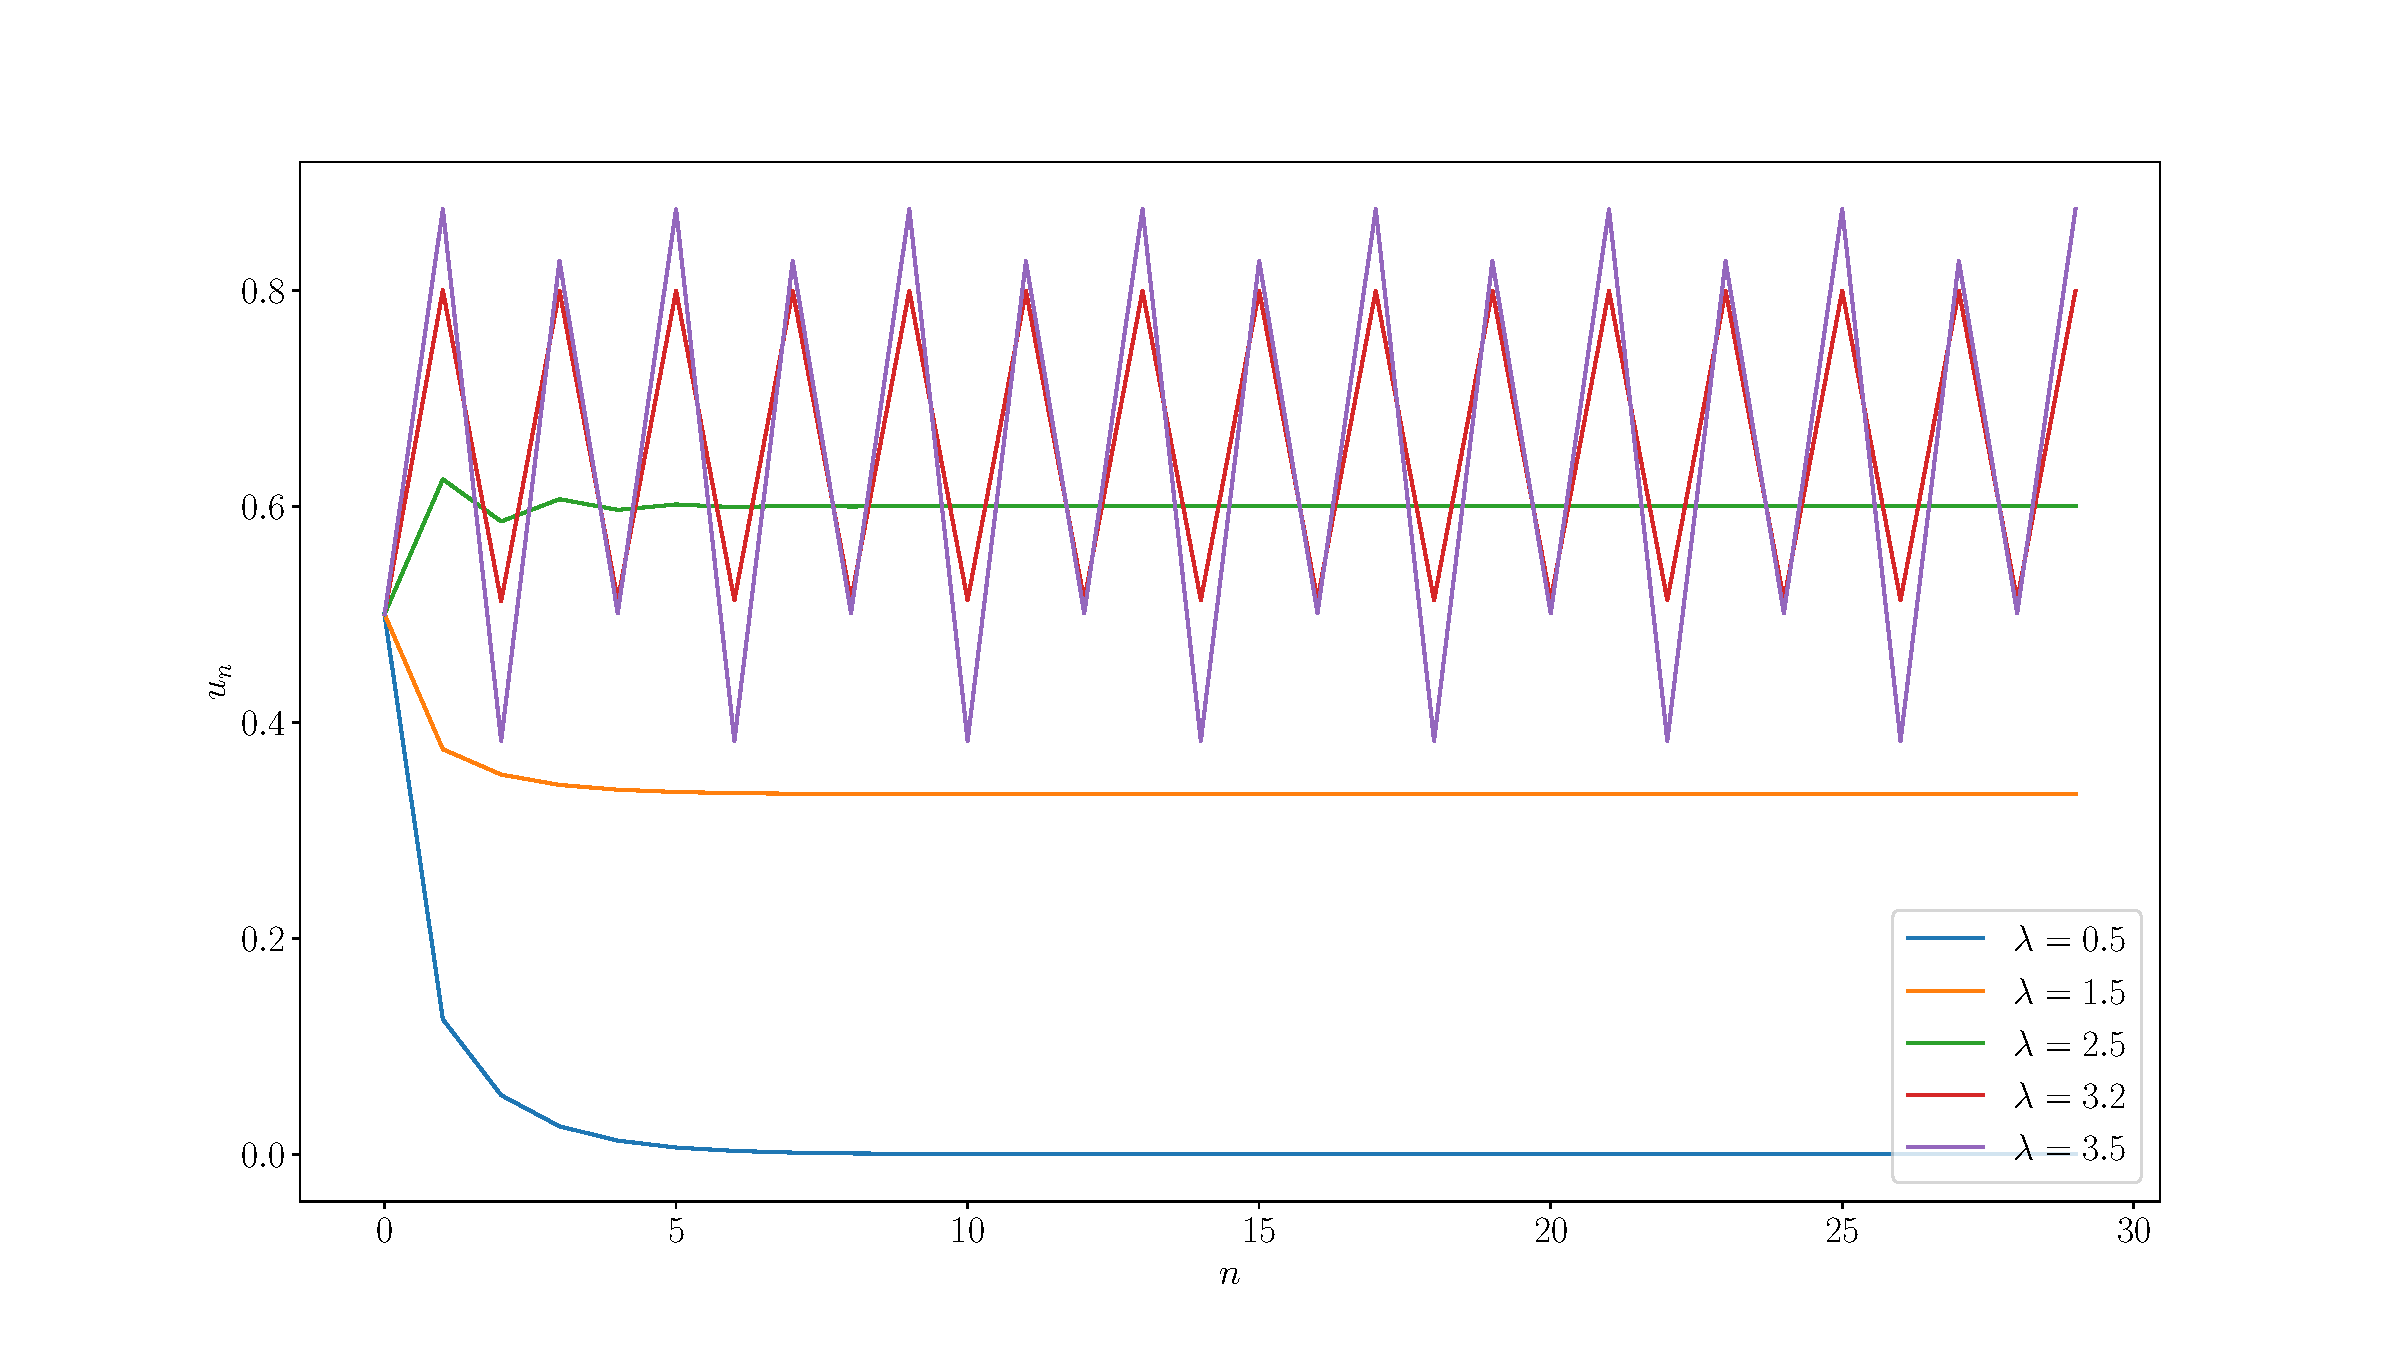
\includegraphics[width=\textwidth]{experimentation_numerique.pdf}
    \end{center}
    \caption{\label{fig:etude_lambdas}Etude de la suite logistique pour différentes valeurs de $\lambda$}
\end{figure}
On peut voir sur la figure \ref{fig:etude_lambdas} que pour les valeurs de $\lambda\in\{0,5; 1,5; 2,5\}$, la suite $(u_n)$ est convergente, et converge respectivement vers (environ) $0; 0,33$ et $0,6$. On peut déceler un comportement particulier pour les valeurs de $\lambda \in\{3,2; 3,5\}$ : elles semblent converger périodiquement vers deux points. On peut trouver les suites extraites afin de donner une valeur approchée de leurs limites.

Pour $\lambda = 3,2$, la suite des termes pairs $(u_{2n})$ converge vers approximativement $0,51$. Tandis que la suite des termes impairs $(u_{2n+1})$ converge vers approximativement $0,80$. De même pour $\lambda = 3,5$ où, les limites des suites extraites sont (approximativement) $0,4$ et $0,9$.

\subsection{Sensibilité aux conditions initiales}
Pour cette partie, fixons $\lambda = 4$ et étudions la suite logistique avec $u_0 = 0,4$ et $u'_0 = 0,4 + 10^{-8}$. On remarque sur la figure \ref{fig:etude_u0} (page \pageref{fig:etude_u0}) que les courbes se superposent parfaitement jusqu'au 17\ieme{} terme. Au delà, les courbes commencent à se dissocier et se dissocient rapidement.

\begin{figure}[!ht]
    \begin{center}
        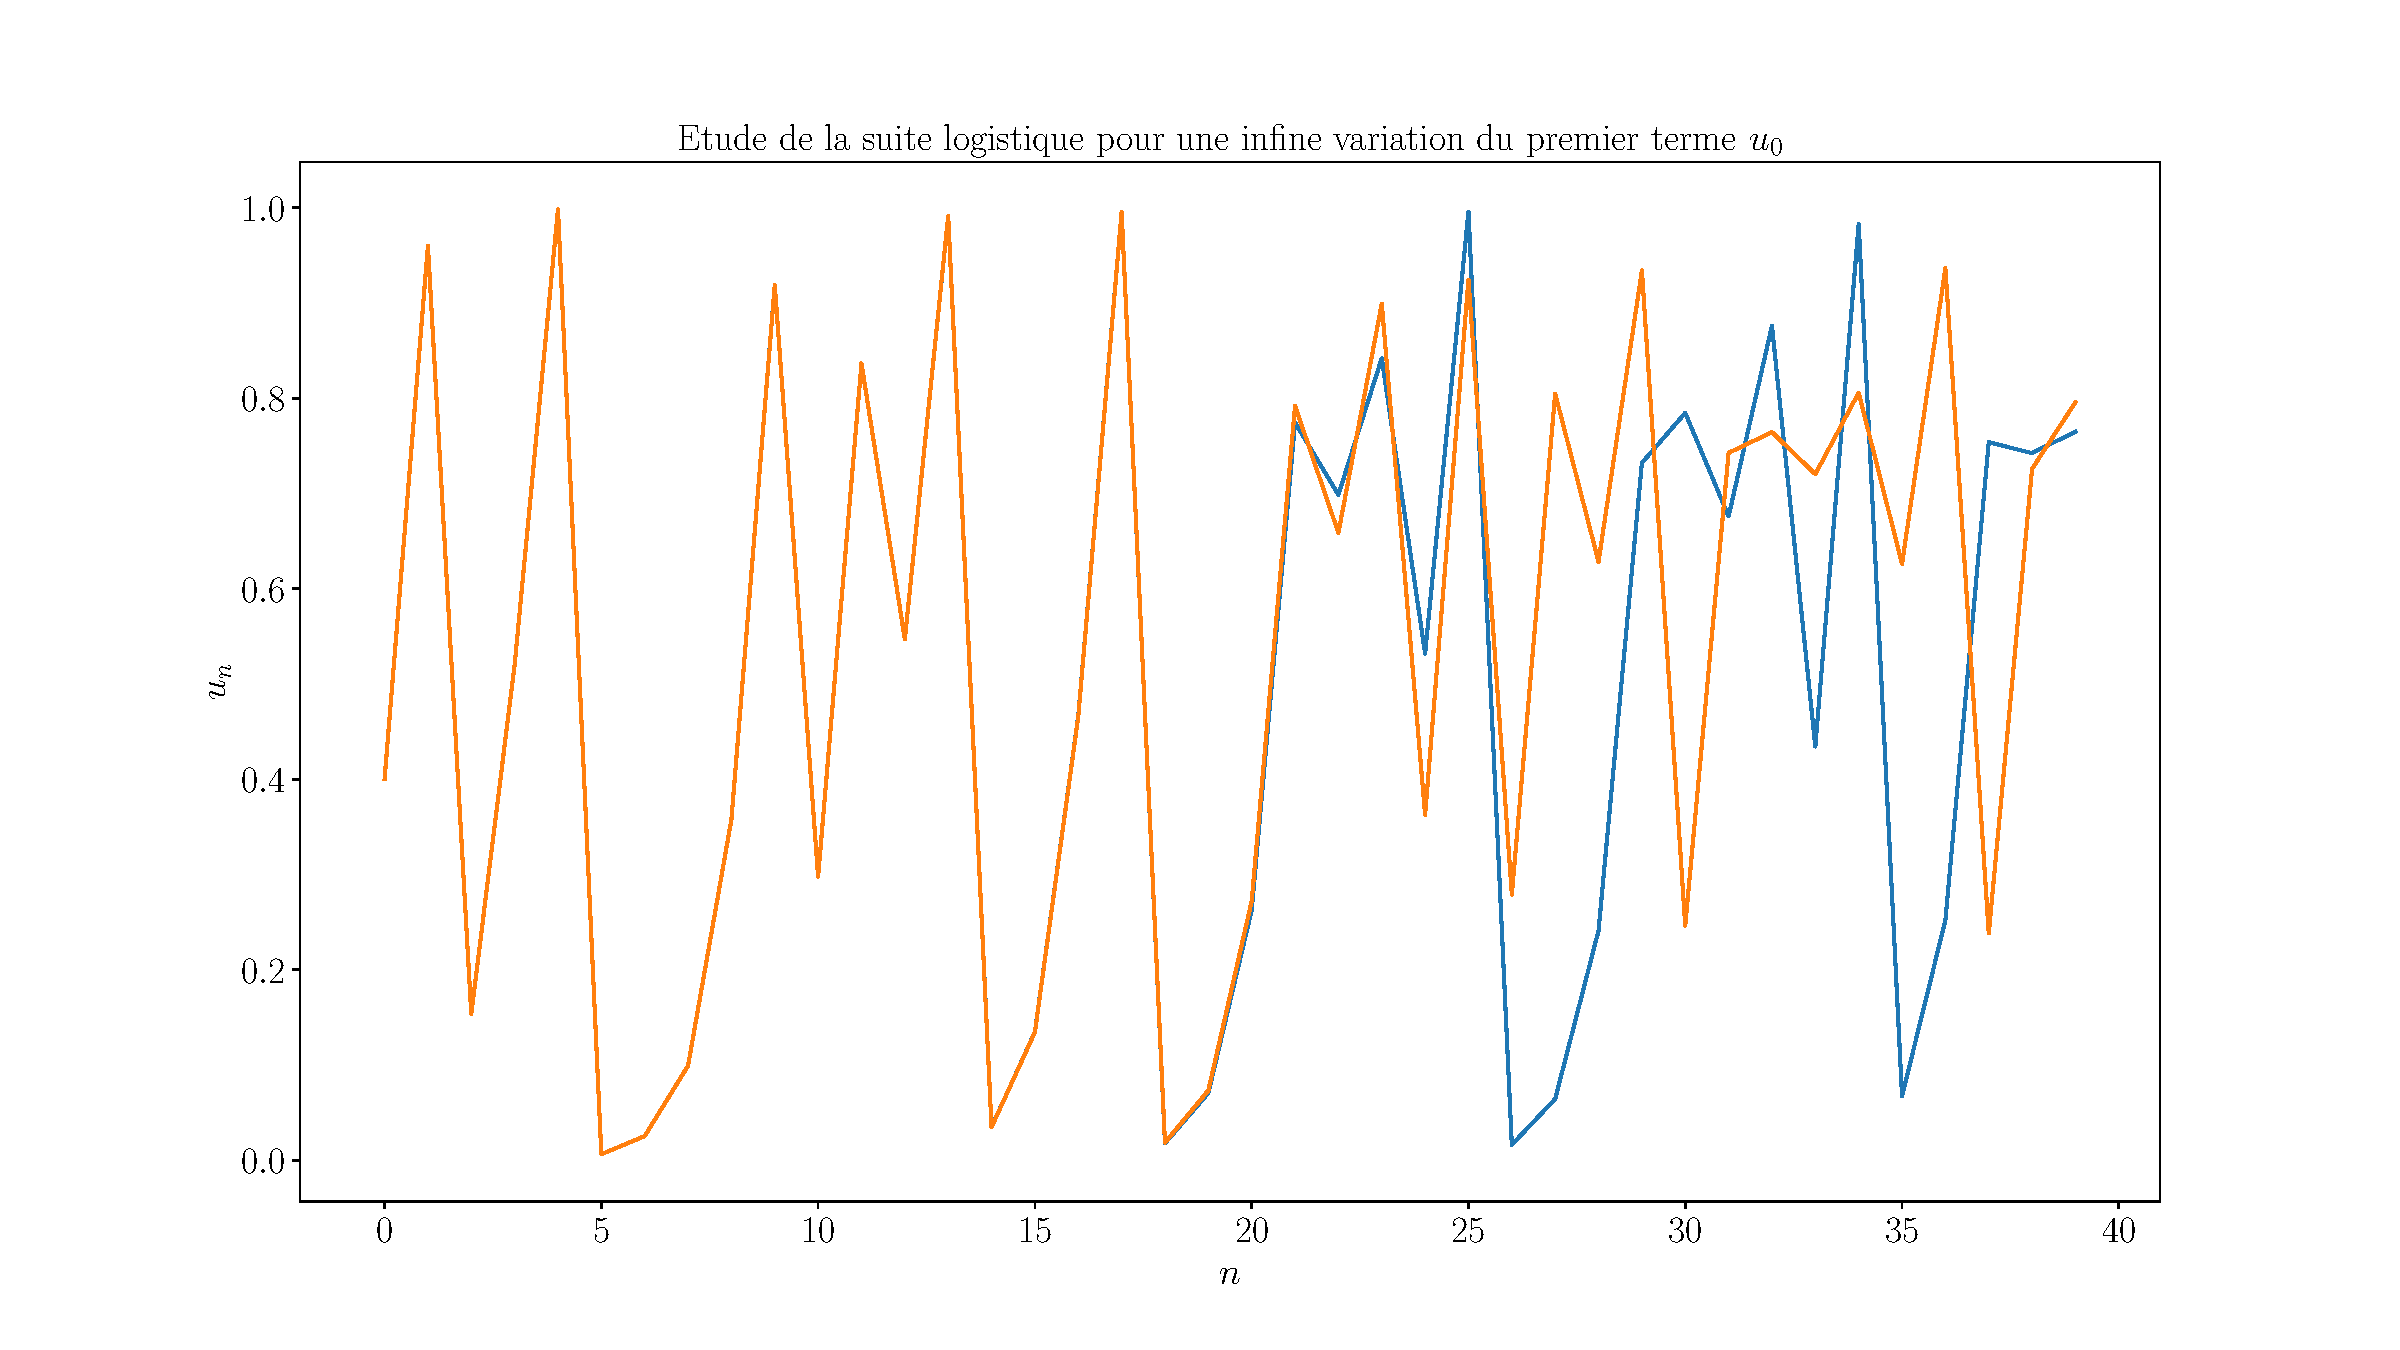
\includegraphics[width=\textwidth]{variation_u0.pdf}
    \end{center}
    \caption{\label{fig:etude_u0}Etude de la suite logistique pour une infime variation du premier terme $u_0$}
\end{figure}

Cette partie illustre le fait que pour $\lambda = 4$, la suite $(u_n)$ a une forte sensibilité aux conditions initiales. Une infine variation des conditions initiales (ici $0,00000001$) a des conséquences énormes sur les résultats : le système est donc \textbf{chaotique}, et introduit la notion d'\textit{effet papillon}.

% Transition

\section{\'Etude mathématique}
\subsection{\'Etude du cas : \texorpdfstring{$\lambda \leq 1$}{Lg}}
\label{section:lambda_1}
Durant toute cette partie, on supposera $\lambda \leq 1$.

En plus des études graphiques, nous allons maintenant nous intéresser à des preuves mathématiques validant les hypothèses que nous aurions pu émettre.
Tout d'abord, nous aurons besoin des bornes de $f_\lambda$ durant toute la suite de l'étude. Montrons donc que $f_\lambda([0;1])\in[0;1]$ :

Etudions la fonction $f_\lambda(x)$ :
\[
    f_\lambda(x)=\lambda x(1-x) = \lambda x - \lambda x^2
\]

Calculons son discriminant $\Delta$ :
\[
    \begin{array}{rcl}
        \Delta &=& \lambda^2-4\times\lambda\times 0 \\
        &=& \boxed{\lambda^2 > 0}
    \end{array}
\]
Il existe donc deux racines $x_1$ et $x_2$ :
\[
    \begin{array}{rcl}
        x_1 &=& \dfrac{- \lambda-\sqrt{\lambda^2}}{-2\lambda} = \dfrac{-2\lambda}{-2\lambda} = \boxed{1} \\
        x_2 &=& \dfrac{- \lambda+\sqrt{\lambda^2}}{-2\lambda} = \boxed{0}
    \end{array}
\]
On voit donc que $f_\lambda$ est \textbf{positive} sur l'intervalle $[0;1]$. Calculons les coordonnées du sommet afin de s'assurer que son ordonnée ne soit pas supérieure à $1$ :
\begin{axiome}[Coordonnées du sommet d'une parabole]
    Soit $f(x) = ax^2+bx+c$ un polynôme du second degré. Les coordonnées du sommet $S$ de la courbe représentative de $f$ sont
    \[
          S\left(-\frac{b}{2a};f\left(-\frac{b}{2a}\right)\right)
    \]
\end{axiome}

Notons, $S_\lambda$ le sommet de la courbe représentative de $f_\lambda$. L'ordonnée de $S_\lambda$ vaut :
\[
    f\left(\dfrac{1}{2}\right) = \dfrac{\lambda}{4}
\]

Calculons les bornes de $y$ en fonction de $\lambda$ :
\[
    \begin{array}{rcccl}
        0 &\leq& \lambda &\leq& 1 \\
        \Longleftrightarrow 0 &\leq& \dfrac{\lambda}{4} &\leq& \dfrac{1}{4}
    \end{array}
\]

Comme $\frac{1}{4} < 1$, le sommet ne dépassera jamais $1$. Donc $\boxed{f([0;1]) \subset[0;1]}$. Cela ne pose pas non plus de soucis lorsqu'on étudie la version discrète à l'aide de suites, car comme $u_0 \in[0;1]$ et que $f_\lambda([0;1])\subset[0;1]$, alors $f_\lambda(u_n) = u_{n+1}\in[0;1]$.


Nous voyons graphiquement que pour $\lambda \leq 1$, la suite semble converger vers $0$. Prouvons cela mathématiquement en étudiant la monotonie de la suite $(u_n)$.
$$
    \begin{array}{rcl}
        u_{n+1}-u_n &=& \lambda u_n(1-u_n)-u_n \\
                    &=& u_n(\lambda(1-u_n)-1) \\
    \end{array}
$$
Or,
$$
    \begin{array}{rcl}
        &&u_n \leq 1 \\
        &\Longleftrightarrow& 1 - u_n \leq 1 \\
        &\Longleftrightarrow& \lambda(1 - u_n) \leq 1 \\
        &\Longleftrightarrow& \lambda(1 - u_n) - 1 \leq 0 \\
        &\Longleftrightarrow& u_n(\lambda(1 - u_n) - 1) \leq 0 \\
    \end{array}
$$
La suite est donc \textbf{décroissante}. De plus, elle est minorée par $0$. Elle est donc bien \textbf{convergente}. Il serait également intéressant de connaître la limite de la suite $(u_n)$, élément crucial afin de déterminer son comportement en fonction de $\lambda$.
\begin{axiome}[Point fixe]
    En mathématique, pour une application $f$ d'un ensemble $E$ dans lui-même, un élément $x$ de $E$ est un \textbf{point fixe de $f$} si
    \[
        f(x) = x  
    \]
    Graphiquement, les points fixes d'une fonction $f$ (d'une variable réelle, à valeurs réelles) s'obtiennent en traçant la droite d'équation $y = x$ : tous les points d'intersection de la courbe représentative de $f$ avec cette droite sont alors les points fixes de $f$.
\end{axiome}
\begin{axiome}[Point fixe et convergence]
    On considère une fonction continue $f : E \longrightarrow E$ et $(u_n)$ une suite récurrente définie par sa valeur initiale $u_0$ et par la relation de récurrence $u_{n+1} = f(u_n)$.
    
    Si $(u_n)$ converge vers un élément $l$ de $E$, la limite $l$ est nécessairement un point fixe de $f$.
\end{axiome}

Afin de trouver la limite de la suite $(u_n)$, nous allons donc calculer les points fixes de $f_\lambda$ pour $\lambda \leq 1$. C'est à dire, résoudre l'équation $f_\lambda(x) = x$:
\[
    \begin{array}{rcl}
        && f_\lambda(x) = x \\
        &\Longleftrightarrow& \lambda x(1-x)-x = 0 \\
        &\Longleftrightarrow& x(\lambda(1-x)-1) = 0 \\
        &\Longleftrightarrow& -\lambda x(-(1-x)+\frac{1}{\lambda}) = 0 \\
        &\Longleftrightarrow& -\lambda x(x-1+\frac{1}{\lambda}) = 0 \\
        &\Longleftrightarrow& -\lambda x(x-(1-\frac{1}{\lambda})) = 0 \\
    \end{array}
\]

Par déduction directe, on peut trouver les solutions de l'équation
$$
    f_\lambda(x) = x \Longleftrightarrow \left\{
            \begin{array}{rcl}
                    x &=& 0 \\
                    x &=& 1 - \dfrac{1}{\lambda}
            \end{array}
        \right.
$$
\vspace{1cm} \\
Cette équation a donc deux solutions : $x_1 = 0$ et $x_2 = 1 - \frac{1}{\lambda}$. Or, $\lambda \leq 1$, donc $x_2 \leq 0$. $x_2$ n'est donc pas un élément de $E$, il ne s'agit donc pas d'un point fixe. Ainsi, pour $\lambda \leq 1$, la fonction $f_\lambda$ possède un unique point fixe sur $[0,1]$ qui est $x = 0$. Nous avons montré précédemment que la suite $(u_n)$ tend vers une limite $l$. Par construction de $(u_n)$ et par continuité de $f_\lambda$, on a 
$$
    \left\{
        \begin{array}{rcl}
                u_{n+1} &=& f(u_n) \\
                u_{n+1} &\longrightarrow& l \\
                f(u_n)  &\longrightarrow& f(l) \\
        \end{array}
    \right.
$$

\begin{wrapfigure}{R}{0.50\textwidth}
    \centering
    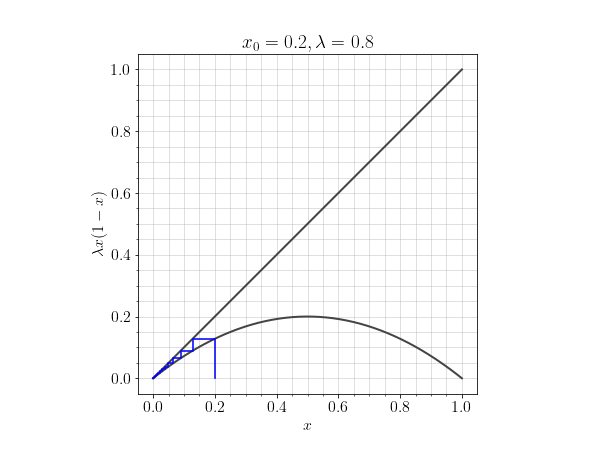
\includegraphics[width=0.49\textwidth]{cobweb_0.2_0.8.png}
    \caption{\label{fig:cobweb_0.2_0.8}$\lambda = 0.8$ et $u_0 = 0.2$}
\end{wrapfigure}
On en déduit donc que $l = f(l)$, c'est-à-dire que $l$ est un \textbf{point fixe} de $f_\lambda$, et $l=0$. La suite (et donc la fonction logistique) tendent bien vers 0, lorsque $\lambda \leq 1$. On peut d'ailleurs voir sur la figure \ref{fig:cobweb_0.2_0.8} (appelé graphique en toile d'arraignée) que l'escalier va au fur et à mesure vers $0$. On dit que $0$ est un \textbf{point fixe attractif}. Cela signifie que dès qu'un terme de $(u_n)$ est dans le voisinage de ce point fixe, tous les termes suivants restent dans le voisignage et la suite converge vers ce point fixe. \'A l'opposé, un point fixe \textbf{répulsif} lorsque $(u_n)$ va s'éloigner du voisignage considéré.

Mathématiquement, un point fixe est attractif lorsque $|f'_\lambda(x_0)| < 1$ et répulsif lorsque $|f'_\lambda(x_0)| > 1$.

\subsection{\'Etude du régime stationnaire : \texorpdfstring{$1 < \lambda < 3$}{Lg}}
\begin{wrapfigure}{R}{0.50\textwidth}
    \centering
    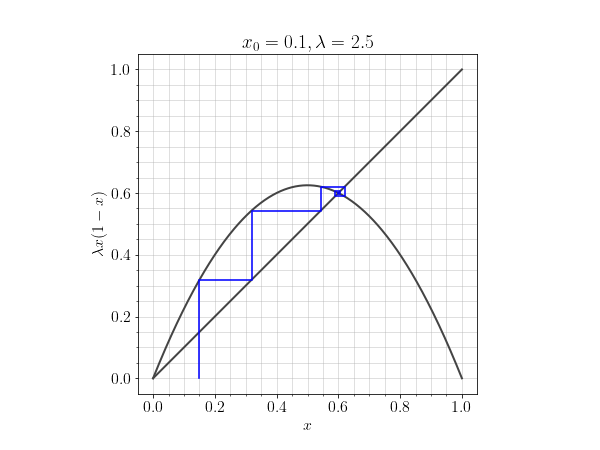
\includegraphics[width=0.49\textwidth]{cobweb_0.1_2.5.png}
    \caption{\label{fig:cobweb_0.1_2.5}$\lambda = 2.5$ et $u_0 = 0.1$}
\end{wrapfigure}
Dans la section précedente, nous avons déterminé les points fixes de $f_\lambda$ suivants : $0$ et $1 - \frac{1}{\lambda}$. Cette fois-ci, pour $1 < \lambda < 3$, nous avons bien $ 0 \leq 1 - \frac{1}{\lambda} \leq 1$. On peut donc noter le point fixe $p_\lambda = 1 - \frac{1}{\lambda}$. La fonction admet donc bien deux points fixes :
$$
    \left\{
    \begin{array}{rcl}
            p_1 &=& 0\\
            p_2 &=& 1 - \frac{1}{\lambda}\\
    \end{array}
    \right.
$$

Intéressons nous maintenant à leur attractivité. Nous voyons bien graphiquement (figure \ref{fig:cobweb_0.1_2.5}) que, malgré le premier terme proche du point fixe $0$, la suite converge vers $0,6$. On peut donc supposer que $0$ est répulsif et $0,6$ attractif. Nous allons calculer mathématiquement les points fixes afin de confirmer cette hypothèse.

$$f'_\lambda(x)=\lambda-2\lambda x\\$$
$$\left\{
    \begin{array}{rcl}
            |f'_\lambda(p_1)| &=& |\lambda| > 1\\[5pt]
            |f'_\lambda(p_2)| &=& |2 - \lambda| < 1\\
    \end{array}
    \right.$$

Donc, $p_1 = 0$ est bien \textbf{répulsif} et $p_2 = 1 - 0,4 = 0,6$ \textbf{attractif}. Ici, nous avons calculé les valeurs avec l'exemple en figure \ref{fig:cobweb_0.1_2.5}. Mais cela est valable pour tout $\lambda$ compris entre $1$ et $3$ (strictement).

\newpage
\subsection{\'Etude d'un cycle d'ordre 2 : \texorpdfstring{$3 < \lambda < 1+\sqrt{6}$}{Lg}}
\begin{wrapfigure}{R}{0.50\textwidth}
    \centering
    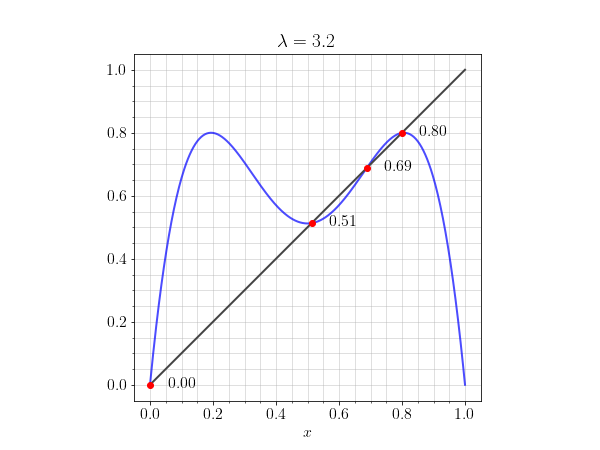
\includegraphics[width=0.49\textwidth]{order_2_cycle_3.2.png}
    \caption{\label{fig:order_2_cycle_3.2}$\lambda = 3,2$}
\end{wrapfigure}
Nous rentrons dans un autre cas pour $\lambda > 3$, car $p_\lambda$ devient \textbf{répulsif}. En effet, si 0$\lambda = 3$, on a $|f'_\lambda(p_\lambda)| = |2-\lambda|<1$. Si nous regardons la figure \ref{fig:etude_lambdas}, nous notons une oscillation entre deux valeurs, cela fait apparaître deux suites extraites convergentes, on dit qu'il y a un \textbf{cycle d'ordre 2} : la suite des termes de rang \textbf{pairs}, et la suite des termes de rangs \textbf{impairs}. Cela entre en cohésion avec le résultat trouvé lors de notre analyse graphique (section \ref{section:version_discrete}).

L'objectif est donc d'étudier les suites $(u_{2n})$ et $(u_{2n+1})$. Or, $u_{2(n+1)} = f_\lambda(u_{2n+1}) = f_\lambda(f_\lambda(u_{2n}))$. De même que $u_{2(n+1)+1} = f_\lambda(f_\lambda(u_{2n+1}))$. On voit donc que l'étude de ces suites revient à étudier $f_\lambda \circ f_\lambda$.

Nous apercevons sur la figure \ref{fig:order_2_cycle_3.2} que $0$ est toujours un point fixe, tout comme $0,69$. Cela fait en effet sens, car les points fixes de $f_\lambda$ sont aussi des points fixes de $f_\lambda^2$. Si $x$ est un point fixe de $f_\lambda$, on a $f_\lambda(f_\lambda(x)) = f_\lambda(x)=x$. En développant $f_\lambda \circ f_\lambda$, nous obtenons le polynôme suivant :

$$-\lambda^3x^4+2\lambda^3x^3-(\lambda^3+\lambda^2)x^2+\lambda^2x$$

On sait que $0$ et $1 - \frac{1}{\lambda}$ sont des points fixes de $f_\lambda^2$. Ce sont donc des racines du polynome
$$P_\lambda(x) = -\lambda^3x^4+2\lambda^3x^3-(\lambda^3+\lambda^2)x^2+(\lambda^2 - 1)x$$

Sont (pour $\lambda = 3,2$):

$$
    \left\{
    \begin{array}{rcl}
            l_1 &=& \dfrac{\lambda + 1 - \sqrt{(\lambda+1)(\lambda-3)}}{2\lambda} = 0,513045\\[10pt]
            l_2 &=& \dfrac{\lambda + 1 + \sqrt{(\lambda+1)(\lambda-3)}}{2\lambda} = 0,799455
    \end{array}
    \right.
$$
Nous retrouvons les valeurs limites obtenues dans la section \ref{section:version_discrete}. Nous pourrions montrer que ces points fixes sont dans $[0;1]$ et qu'ils sont stables.

\newpage
\section{Le diagramme de bifurcation}
Si nous continuons d'augmenter $\lambda$, on obtient des cycles d'ordre 4, puis 8, etc\dots (Voir annexe \ref{ann:cycles}). On parle de cascade de doublement de période
Nous allons donc nous intéresser aux valeurs de passages à l'ordre de multiplicité 2 supérieur. Nous allons pour cela représenter un diagramme de bifurcation. Ce diagramme \textbf{représente la/les valeur(s) du/des point(s) fixe(s) en fonction de la valeur de $\lambda$}.

\begin{figure}[!ht]
    \begin{center}
        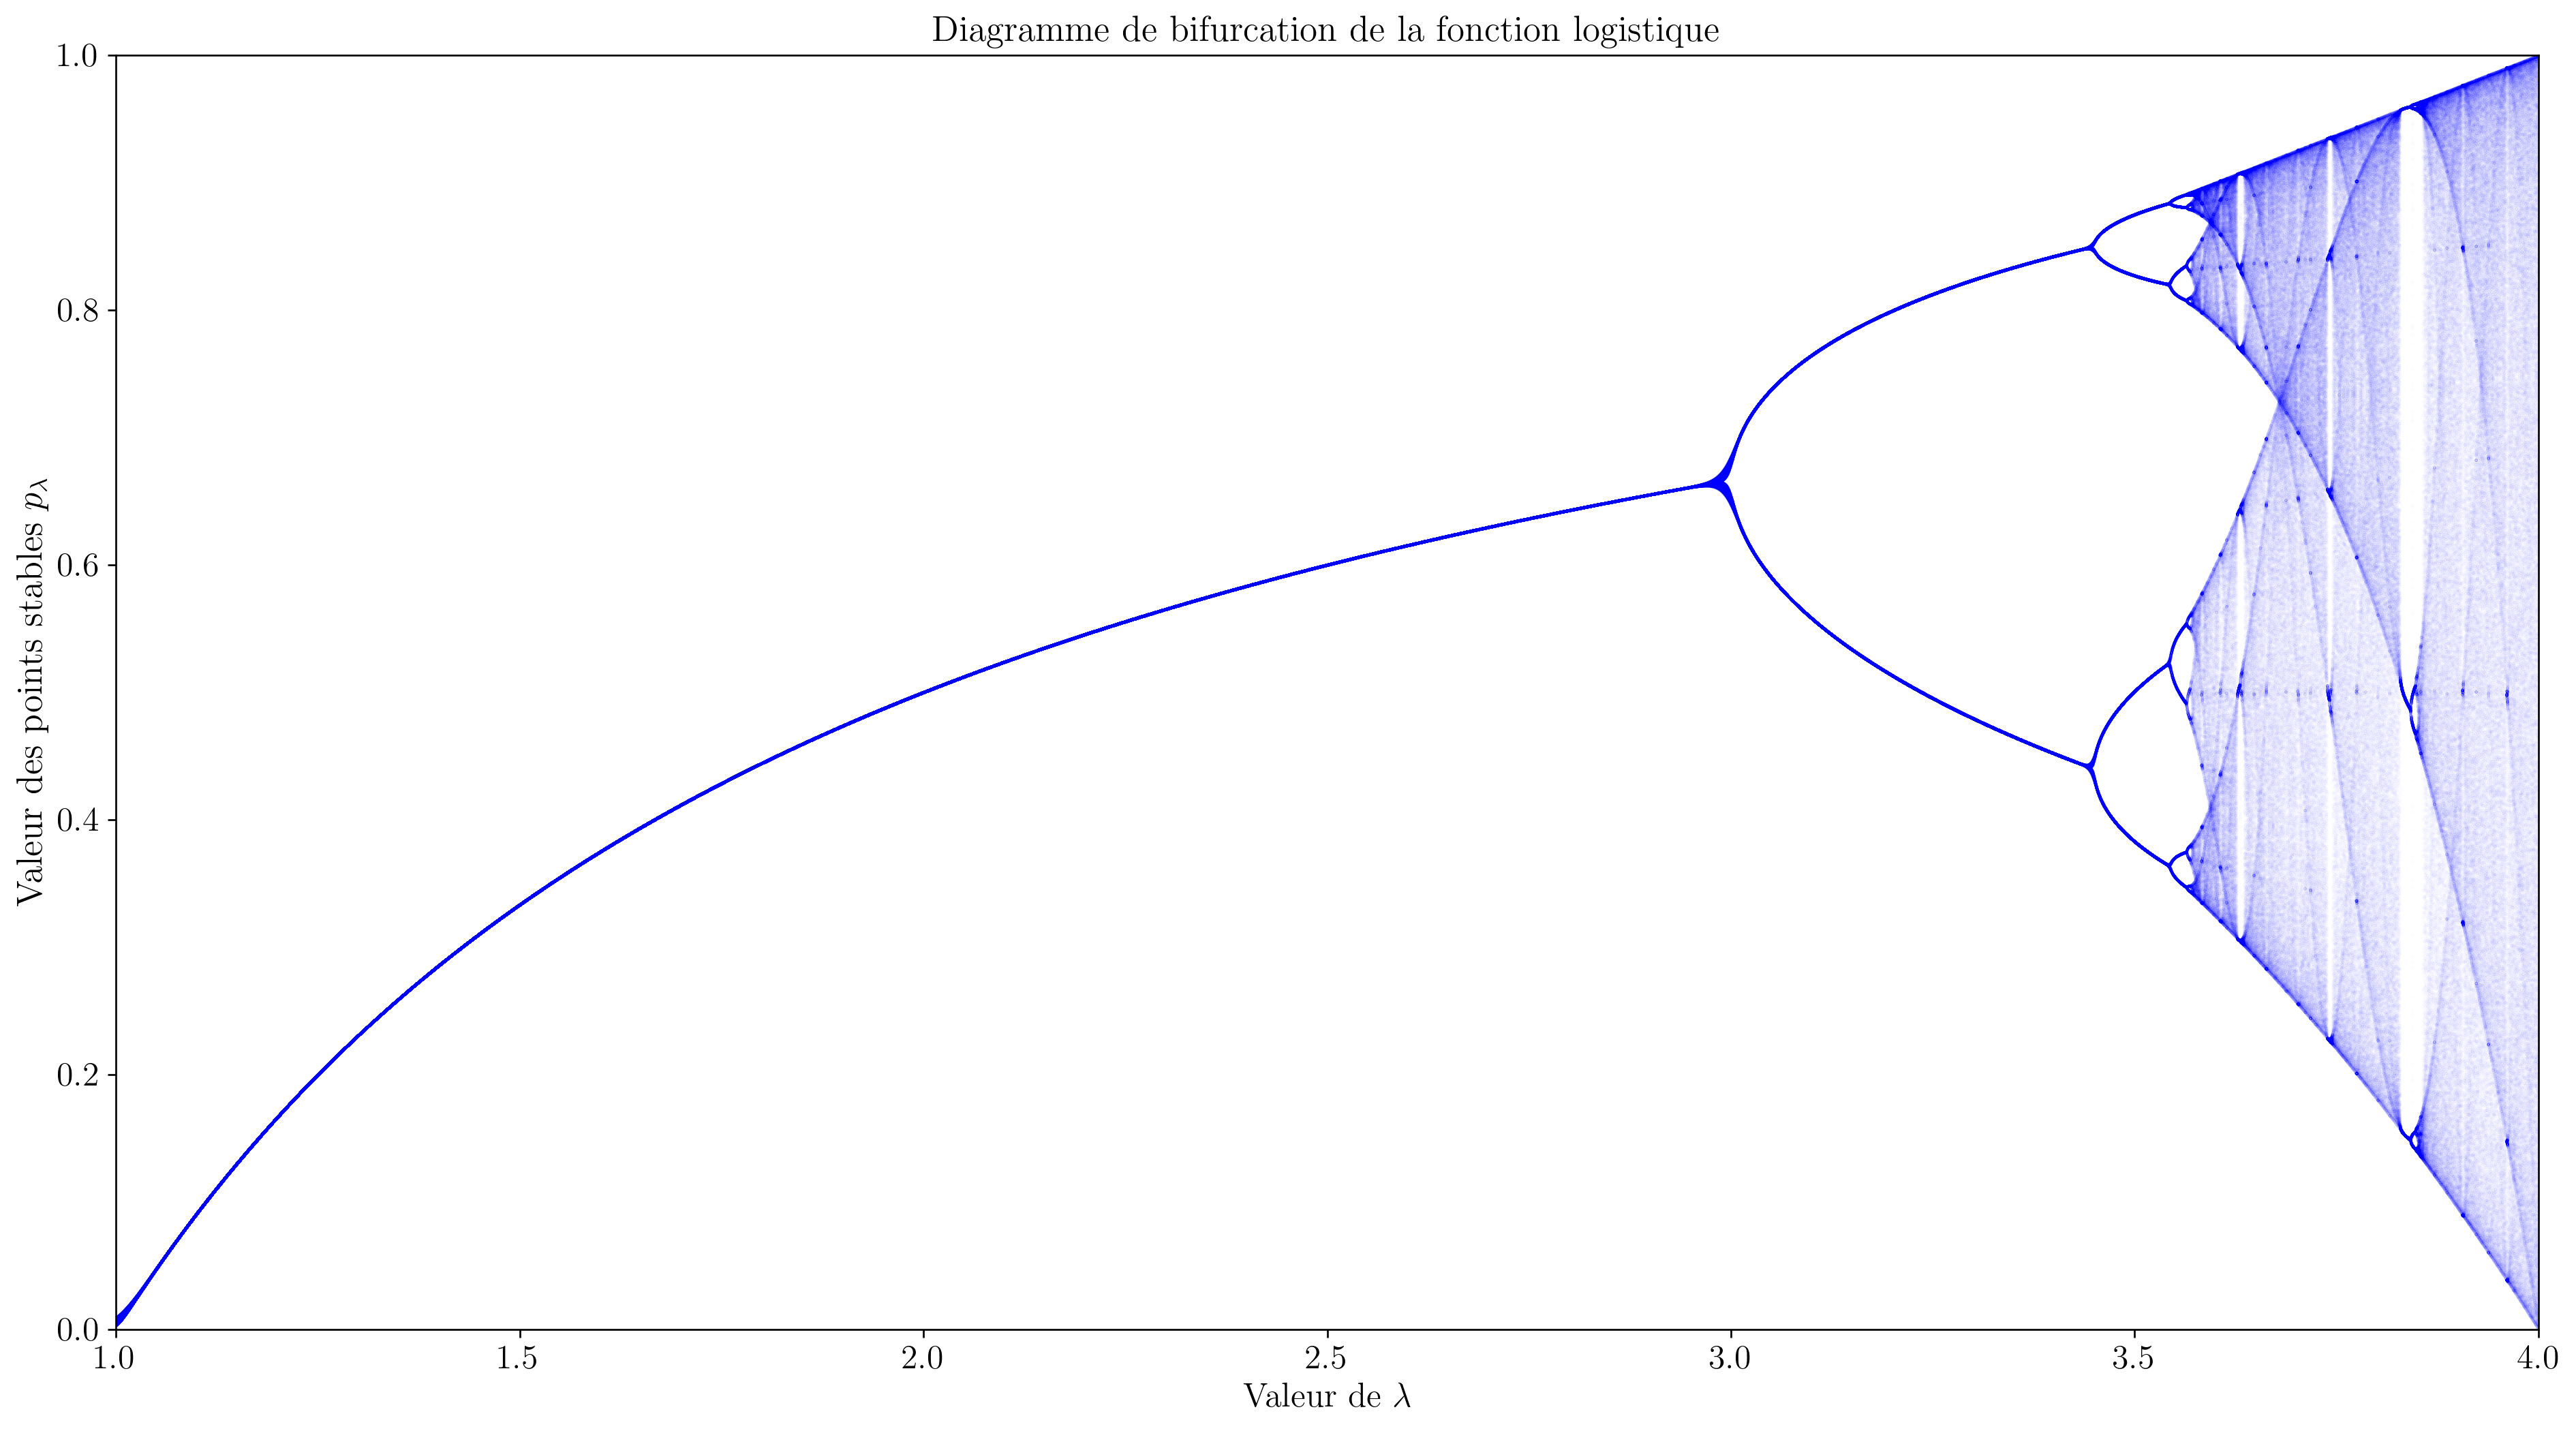
\includegraphics[width=\textwidth]{bifurcation.png}
    \end{center}
    \caption{\label{fig:bifurcation}Diagramme de bifurcation de la fonction logistique}
\end{figure}

Cela est cohérent avec ce que l'on a trouvé dans les parties précedentes. On peut cependant noter un changement brutal de comportement à partir de $\lambda = 3.57$. On entre dans un comportement complètement chaotique, sans aucune orbite périodique.
